%\section{「振り返る」機能}
振り返る機能は観光中にユーザが撮影した写真もしくはデフォルトでアプリ内に入っている写真を対応するスポットの紹介文と共にスワイプ操作で見ることができる機能である。撮影した写真とデフォルトの写真の表示切替は、画面右上にあるタブをタップすることでできる。また、ユーザが撮影した写真が1枚もない場合も考えられるためno imageなどの表示ではなく、木古内町マスコットキャラクター「キーコ」がお辞儀をしている画像と、写真を撮ると表示される旨のメッセージをカードリスト画面の雰囲気と統一をさせて表示した。\par
本機能には、スワイプできることが伝わらないということや全部で何枚の写真があるのかが分からないという問題が現状では存在する。それらに対して、矢印を左右に表示したり``pagecontrol"という図6.5のような何個中何個目という情報を表示できる部品を活用する案があった。しかし、画面上にスワイプ操作ができるという矢印を表示した場合の画面レイアウトを期間中に考案することが困難だったため、現状のままとしている。また、``pagecontrol"については写真の枚数が膨大になることで対応しきれない可能性があるため実装を行わなかった。

\newpage

\begin{figure}[htbp]
  \begin{center}
    \begin{tabular}{c}

      % 1
      \begin{minipage}{0.33\hsize}
        \begin{center}
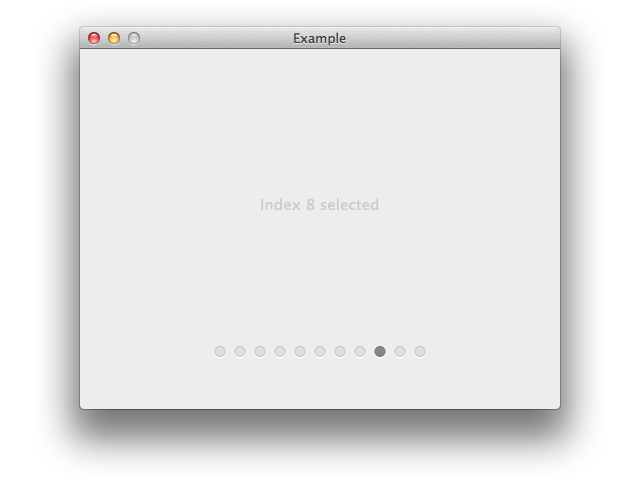
\includegraphics[width=4cm, bb=0 0 640 480]{pagecontrol.png}
       %   \hspace{1cm} pagecontrolのサンプル
        \end{center}
      \end{minipage}

    \end{tabular}
    \caption{pagecontrolのサンプル}
    \label{fig:lena}
  \end{center}
\end{figure}

\begin{figure}[htbp]
  \begin{center}
    \begin{tabular}{c}

      % 2
      \begin{minipage}{0.33\hsize}
        \begin{center}
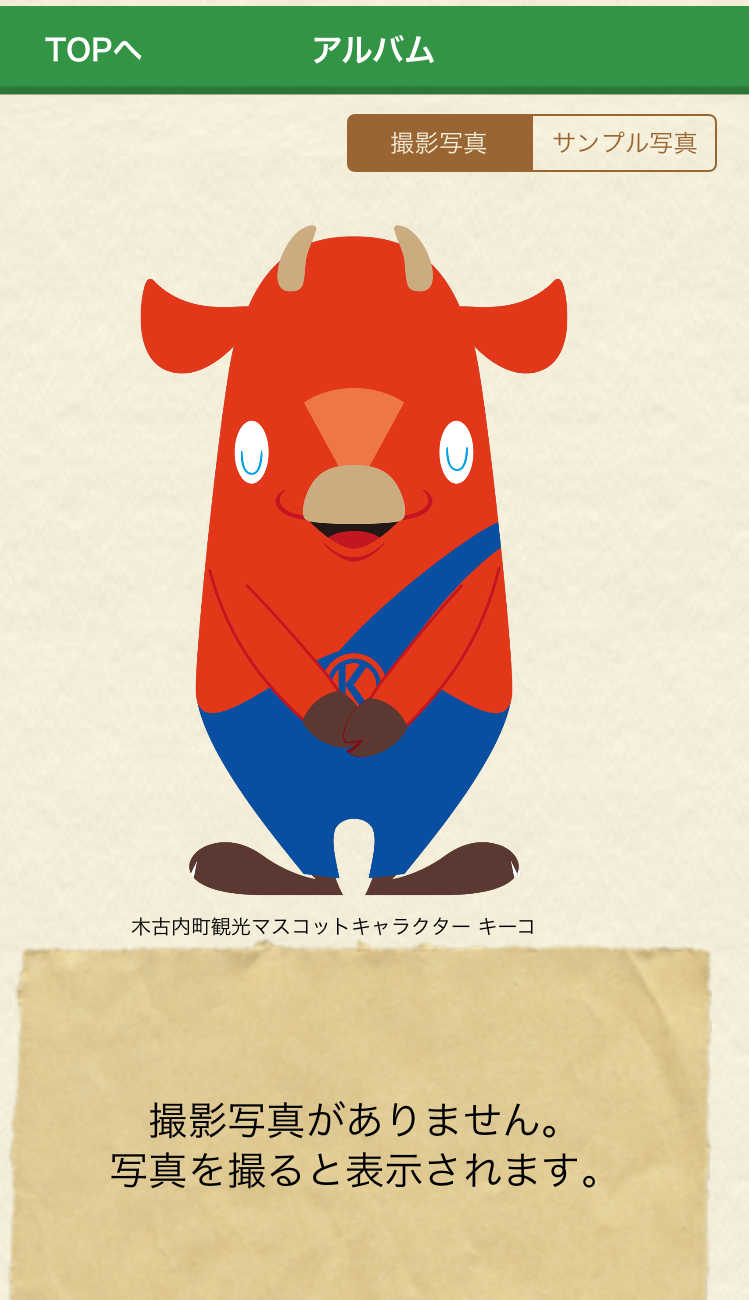
\includegraphics[width=4cm, bb=0 0 304 570]{album1.png}
          \hspace{1cm} (a)撮影写真なしの表示例
        \end{center}
      \end{minipage}
      
            % 3
      \begin{minipage}{0.33\hsize}
        \begin{center}
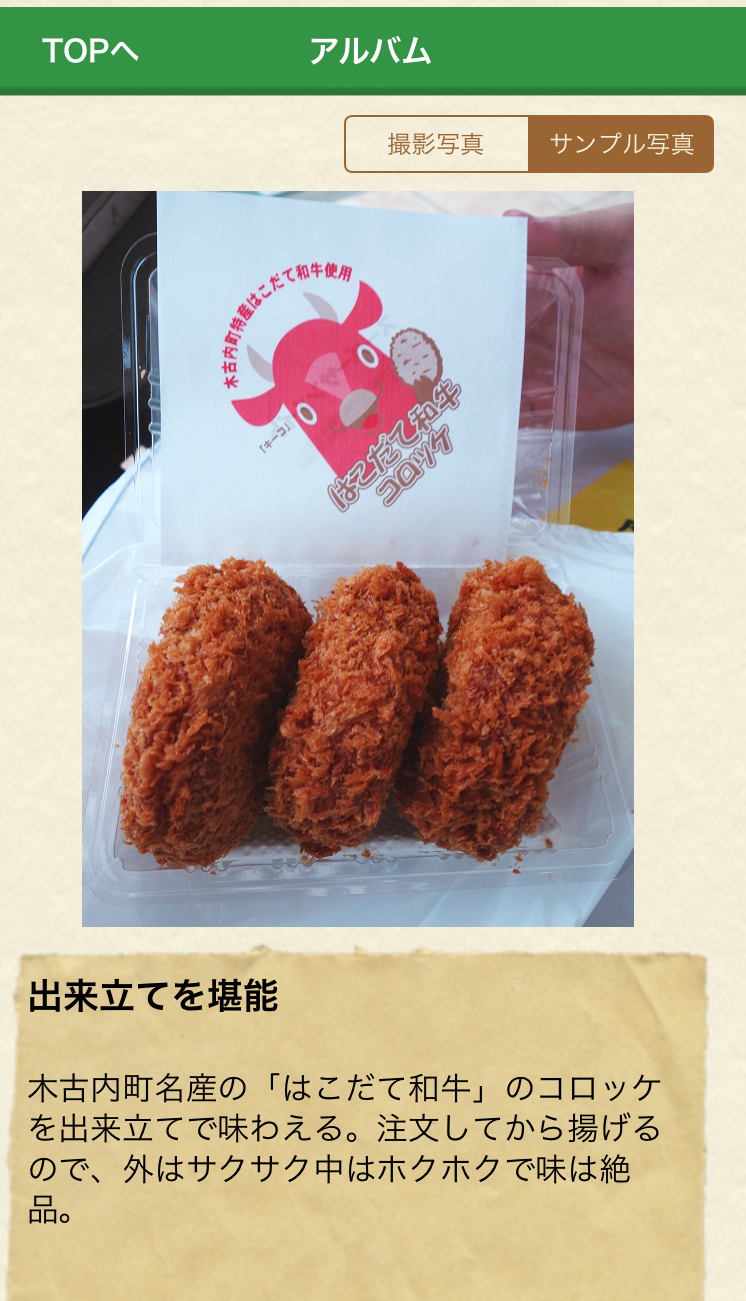
\includegraphics[width=4cm, bb=0 0 304 570]{album2.png}
          \hspace{1cm} (b)振り返る機能の表示例
        \end{center}
      \end{minipage}

    \end{tabular}
    \caption{振り返る機能の画面}
    \label{fig:lena}
  \end{center}
\end{figure}                                                                                                                                   \bunseki{岩見建汰}